\documentclass[11pt]{article}
\usepackage{graphicx, amssymb,amsmath,cite}
%\usepackage{uspstyle}
\usepackage{tda,trimspaces}
\bibliographystyle{plainurl}


\begin{document}

\maketitle



\section{Introduction}
% Provide a statement of the objective(s) and the anticipated significance of the 
% work to your field of study. What problems will be investigated? What hypothesis 
% will be tested? We suggest that the introduction begin with a brief description 
% of the project in general terms before the more technical aspects of the project 
% are discussed. 
\todo{I made some changes!}

The problem of finding the minimum area of a null homotopy of a closed curve in the plane has a rich history and a bright future. Chambers and Wang ~\cite{cw2013} gave a polynomial algorithm to find the minimum homotopy of simple curves. Fasy, Karako\c{c} and Wenk ~\cite{fkw2017} gave an exponential algorithm for computing the minimum homotopy of normal curves. In an unpublished preprint Nie ~\cite{nie2014} gave a polynomial algorithm to compute the minimum area homotopy between two closed plane curves using an algebraic argument. Nie does not give an explanation of how to generate a word from a given curve. In this work we give a polynomial algorithm for inputting a curve into Nie's algorithm. We also give a geometric description of the minimum homotopy produced in terms of collections of Jordan curves. 


%Figure~\ref{fig:TODO-name}


% \begin{figure}
%  \centering
%  \includegraphics[height=1.25in]{TODO:relative-path}
%  \caption{TODO.}\label{fig:TODO-name}
% \end{figure}

\section{Background}
% Provide a brief review of the work that has been done in the project 
% area together with complete references in appropriate professional style. This 
% section should also include any personal information about you that would 
% indicate to the reviewers your qualifications for successfully completing this 
% project, including a statement of how the project will contribute to your 
% academic and career goals.
\todo{What needs to be included here?? OK ok}


An introduction to the minimum homotopy problem is given in \cite{fkw2017}. In section 2 of ~\cite{nie2014} the weighted cancellation norm on the free group is defined. Theorem 4.1 of~\cite{nie2014} proves that the minimum area of a homotopy between two curves $\gamma_1$ and $\gamma_2$ exists, and is equal to the weighted cancellation distance of the words generated by the curves. If we let one of the curves be a point we have solution to the minimum null homotopy problem. 

\section{Generating words from curves}


% Provide a detailed description of the research methods that you will 
% use in the project. This should include a justification for the specific 
% approach that you will use. For example, how do the methods answer the questions 
% that have been posed, test the hypothesis, or lead to the desired goal?
% Timeline: Provide dates for the initiation and completion of each phase of the 
% project. Attempt to lay out a reasonable schedule taking into consideration all 
% phases of the research and final deliverables.

\todo{This needs to be justified or changed to a conjecture}

We now give a algorithm that, when given a closed curve generates a word such that the weighted cancellation norm of the word gives the minimum null homotopy area. Our algorithm is quadratic in the number of regions of the curve.

To this end let $C$ be closed curve in the plane and $P_C=\{p_0,p_1,...,p_n\}$ the set of anchor points. Let T be a spanning tree of $P_C.$ T is null homotopic. Consider the homotopy that contracts T to a point and preserves the area of each region. Call the resulting curve F. F only has a unique point and each region in F is bounded by a single edge, see Figure \ref{Figure 1}. We notate a region by $a,$ its area by $|a|$ and its single edge by $e_a.$

Note that there are potentially several trees $T$ that can be chosen if $C$ contains one or more regions with two edges. When traversing a region with sub regions the order of some generators could be swapped depending on the choice of the tree. The cancellation norm of these words is the same.  \todo{needs justification. Hatcher?}.



To generate a word from $C$ pick an anchor point $p_i$ and begin traversing $C.$ As one traverses C the regions in F will be traced out one at a time. When an edge in F is traversed append the generator of that region to the word $w.$ If the region $a$ contains a sub region, $b$ append $b$ to the word after $a$. If $b$ is oriented in the opposite direction as $a$ append $b^{-1}.$ If the region contains more than one sub region include them in the order they appear in $F.$ If a different initial point is selected we will generate a cyclic permutation of our word with an equal cancellation norm.

If a region $a$ has sub regions as in Figure 1, the curve $F$ can be split at $p$ with $e_a$ being the wrap split and the sub curves as the direct split as in definition 2.3 in \cite{parkerThesis}. The curves that make up the exterior of the direct split are added to the word after $a$ with inverses when $e_a$ is oriented in the opposite direction. This process might continue if there are more sub regions but there are a finite number of regions so the process will terminate.


The length of the word is quadratic in the number of regions of $C$. When an edge is traversed the number of generators that are appended to the word is at most the number of regions. This bound can be achieved by a  curve consisting of concentric circles.

When we perform the cancellation norm of a word the word is broken into sub sections. Each of these sub section an be viewed as a copy of the corresponding region. These regions appear to always be contractible to points. And the sub sections of the word often give visual clues to what the minimum homotopy looks like. We plan to explore the geometry of these regions in future work.




\begin{figure}
  \centering
  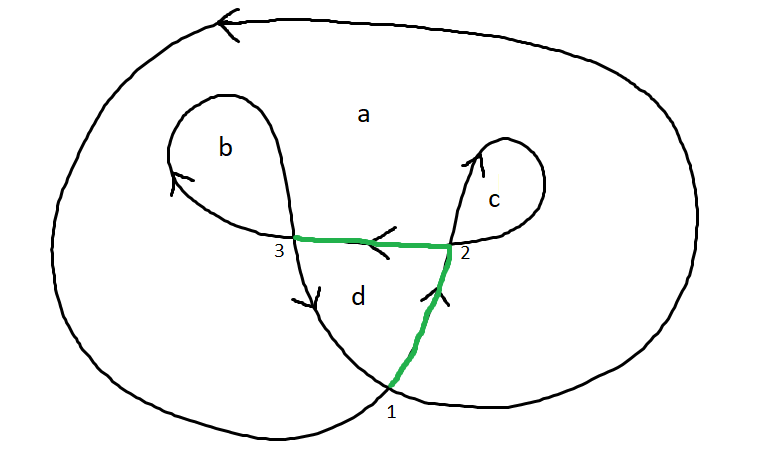
\includegraphics[height=1.25in]{Mouse1.png}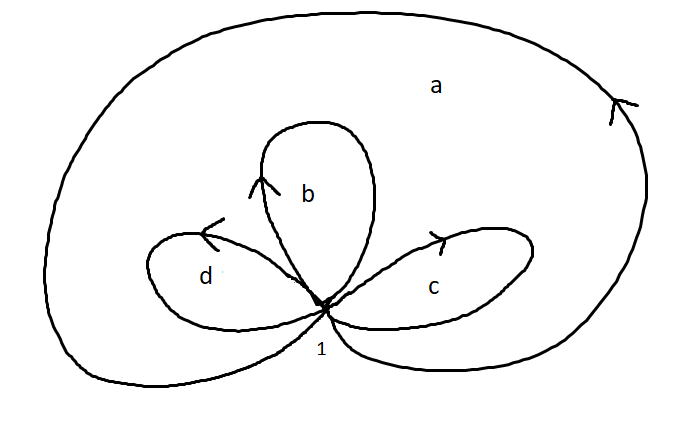
\includegraphics[height=1.25in]{Mouse3.png}
  
  
 (a) \hspace{5cm}(b)
  \caption{(a) is a curve C. The tree T is shown in green. When T is contracted to a point the result is a curve F in (b).}\label{Figure 1}
 \end{figure}
\section{Example}

In this section, we apply our algorithm to generate the  word for the curve in Figure \ref{Figure 1}. First we pick a spanning tree, $T=\overline{p_1,p_2}\cup\overline{p_2,p_3}.$ Contracting $T$ to a points yields $F$ in Figure 1b. Suppose we start at $p_1$ and travel around the region $a$ first. We append $a$ to our word. $a$ has sub regions so we append their generators after $a$. $e_c$ and $e_b$ are oriented in the opposite direction as $e_d$ so they are appended as inverse elements. To traverse $a$ in $C$ our word is $ac^{-1}b^{-1}d.$ We now traverse $c,$ $b$ and finally $d.$ Our word $w$ is $w=ac^{-1}b^{-1}dcbd$. We now compute the minimum cancellation of $w.$ There are two possible cancellations, cancel $b^{-1}$ with $b$ or cancel $c^{-1}$ with $c.$ Since $b$ has larger area than $c$ we cancel $b^{-1}$ and $b.$ The minimum homotopy area of $C$ is then $2|d|+2|c|+|a|.$

The cancellation splits $w$ into three disjoint parts separated by the canceled terms $ac^{-1}, dc$ and $d.$ \todo{make images of these}. Each of these regions is a collection of Jordan Curves. We can use these sub sets of $w$ to visualize the minimum homotopy in the following way. Sweep out region $d$ by deforming $\overline{p_3,p_1}$ onto $\overline{p_1,p_2,p_3}.$ Then contract regions $c$ to $p_1$ and sweep back over $d.$ Finally contract regions $d$ and $b$ around region $a.$


% Please draft your proposal in a format that is appropriate for your academic 
% discipline (i.e. MLA, APA, etc.) - consult your mentor if you have questions 
% about what format is most appropriate to your field of study
%%%%%%%%%%%%%%%%%%%%%%%%%%%%%%%%%%%%%%%%%%%%
%% BIBLIOGRAPHY
 \newpage

 \bibliography{references}
%%%%%%%%%%%%%%%%%%%%%%%%%%%%%%%%%%%%%%%%%%%%




\end{document}